\section{Experiments and Evaluation} 
\label{sec:evaluation}
In this chapter we show and discuss the results of training the outlined neural network architecture for spoken language identification. We introduce several performance metrics and present the results evaluated on our system.
Further, we experiment with modified model architectures to optimize our model for noise robustness. To assess the real world performance of the neural network we augment our data to simulated various noisy environments. We show the classification performance of our approach by discussing the inter language discrimination and extensibility to other languages.     

\subsection{Setup} 
\label{sec:setup}

\subsubsection{Hardware Resources}
\label{sec:hardware}
	In order to facilitate Keras' and TensorFlow's hardware-accelerated computation we ran of training on CUDA\footnote{\url{https://developer.nvidia.com/cuda-zone}, accessed 30.01.2017} compatible \ac{gpu} machines. All trainings and experiments were executed on two CUDA enabled machines belonging to the Internet Technologies and Systems chair. Details can be found in table \ref{tab:hardware}.
		
	\begin{table}[h]
	\centering
	\begin{tabularx}{\textwidth}{lll}
	\toprule
	  		& Machine A 					& Machine B \\ \midrule
	OS  	& Ubuntu Linux 14.04 		& Ubuntu Linux 16.04 \\
	CPU  	& Intel\textsuperscript{\textregistered} Core\textsuperscript{\texttrademark} i7-4790K @ 4GHz 	& AMD FX\textsuperscript{\texttrademark}-8370  @ 4GHz \\
	RAM  	& 16GB 						& 32GB \\
	GPU  	& Nvidia GeForce\textsuperscript{\textregistered} GTX 980 	& Nvidia Titan X \\
	VRAM  	& 4GB 						& 12GB \\
	\bottomrule
	\end{tabularx}
	\caption{Hardware resources used in training the neural network.}
	\label{tab:hardware}
	\end{table}

\subsubsection{Data} 
\label{sec:data}
For our performance evaluation we used the European Speech Repository and YouTube News dataset as describe in section \ref{sec:datasets}. Both datasets were preprocessed and converted spectrogram images as described in section \ref{sec:data_processing}. Each spectrogram image represents a non-overlapping ten second duration of source audio file. 
We split both dataset into a training (70\%), validation (20\%) and testing set (10\%) and all files were distributed equally between all four language classes. The amount of samples per language is limited by language with least files to ensure an equal class distribution. The yield of the datasets could be increased by increasing the number of Spanish files. Nonetheless, the European Speech repository yields a total of 19.000 training images files which adds to roughly 53 hours of speech audio. The YouTube News dataset is considerable larger and yields a total of 194.000 training files, or 540 hours. Table \ref{tab:data_splits} contains the detailed dataset splits.

	\begin{table}[]
	\centering
	\begin{tabularx}{\textwidth}{lrr}
	\toprule
	  				& European Speech Repository & YouTube News\\ \midrule
	Training Set    & 18.788						 & 193.432 \\
	Validation Set  & 5.372						 & 55.272 \\
	Test Set        & 2.684						 & 27.632 \\
	\midrule
	Total           & 26.844						 & 276.336 \\
	\bottomrule
	\end{tabularx}
	\caption{The amount of samples for our training (70\%), validation (20\%) and testing (10\%) set for the respective datasets.}
	\label{tab:data_splits}
	\end{table}

Given the European Speech Repository's smaller size we only used it initially confirm the validity of our approach. Since we were satisfied with the results we did not do include it in the extensive robustness tests that we used for the evaluation on the YouTube News dataset. In addition to the original audio we augmented the news dataset with three different background noises to evaluate how well our model would hold out in non ideal, real world situations outside of a new broadcasting studio. For the first experiment we added generic white noise to data. For the second experiment we added noise to simulate an old phone line or bad internet connection during voice chat. Lastly, we added background music to the data. All experiments are described in detail below.


\subsubsection{Training of the Neural Network Model} 
\label{sec:training}
Neural networks have a multitude of hyperparameters that influence the training results drastically. In the following we will briefly explain our choice of hyperparameters and other important training settings.

	\begin{description}
	\item[Optimizer] We employed an Adam\cite{kingma2014adam} optimizer to quickly and efficiently convergence our model. The Adam solver utilizes momentum during gradient updates and to support a quicker convergence. We set the optimizer's parameters $\beta_1$ to 0.9, $\beta_2$ to 0.999, and $\epsilon$ to 1e-08. Overall we found it to be an order of magnitude quicker than using standard stochastic gradient descent (\ac{sgd}). We resorted to SGD finetuning when we needed more control over the learning rate schedule and wanted smaller weight updates.
	\item[Weights Initializer] All layer weights are initialized within the range [0, 1) using Keras' default random Glorot uniform initializer\cite{glorot2010understanding}.
	\item[Data Normalization] The greyscale images are loaded using SciPy and normalized to the [0, 1] range. The shape for all inputs needs to be uniform across all samples and is set to [500, 129, 1], unless otherwise noted. The data loader uses Python generators\footnote{\url{https://docs.python.org/3/glossary.html#term-generator}, accessed 30.01.2017} to keep the system's memory requirements low.
	\item[Learning Rate] We set the initial learning rate to 0.001. Given the Adam optimizer's dynamic learning rate adaption we expect the learning rate to be increase or decreased after every epoch. 
	\item[Batch Size] We specified the batch size depending on the available VRAM of the training machine. We used a value of 64 for Machine A and 128 for Machine B. See section \ref{sec:hardware} for the hardware specifications. 
	\item[Weight Regularization] We employed the L2 norm as a weight regularizer for all convolutional and fully connected layers to improve the models generality. We penalize our loss with a weight decay value of 0.001. 
	\item[Epochs] We limited the model training to a maximum of 50 epochs when using the Adam solver. We usually reach convergence well below this threshold. For training sessions with SGD we increased this considerably. To speed up our workflow we employed an early stopping policy and stopped a training if the validation accuracy and loss did not increase within a ten window.
	\item[Metrics] We observed the loss, accuracy, recall, precession, f1 measure, and equal error rate for both the training and validation set during model training. All values were saved to log files and visualized as graphs in TensorBoard.  
	\item[Loss] As is common for multivariate classification all models were trained with a softmax cross-entropy loss function.
	\end{description}


\subsection{Evaluation} 

\subsubsection{Evaluation Metrics} 
\label{sec:metrics}
In this section we discuss the evaluation metrics used throughout our experiments. All metrics are generally only defined for binary classification results. Given our multi-class prediction problem we will report the average of the individual class performance measure in the following sections. 

\begin{description}
    \item[Accuracy] is a common measure in machine learning and is defined as the ration of correctly classified samples to all samples in the dataset. In the context of language identification this translates as:
     
    	$$
		Accuracy = \frac{\abs{\{\text{correctly identified language samples}\}}}{\abs{\{\text{all language samples}\}}}
		$$
     
    
    \item[Precision and Recall] Precision defines the ratio of retrieved language samples that are correctly identified as belonging to said language. Recall is the fraction of correctly identified language samples to all samples belonging to this language.
     
		$$
 		truePositives = \abs{\left\{\parbox{0.7\textwidth}{samples belonging to a language which were correctly identified as belonging to said language}\right\}} 
		$$
		
		$$
 		falsePositives = \abs{\left\{\parbox{0.7\textwidth}{samples belonging to a language which were identified as belonging to another language}\right\}}  
		$$
		
		$$
 		falseNegatives = \abs{\left\{\parbox{0.7\textwidth}{samples belonging to a language which were incorrectly identified as not belonging to said language}\right\}}  
		$$

	    $$
	    precision = \frac
	      {truePositives}
	      {truePositives + falsePositives}
	    $$
		
		$$
		recall = \frac
			{truePositives}
			{truePositives + falseNegatives}
		$$    


    \item[The F1 Score] is the scaled harmonic mean of precision and recall. It is used to a have combined judgement of recall and precision, since one is generally not interested in assessing one without the other.
    
    	$$
    	F1 = 2 * \frac{precision * recall}{precision + recall}
    	$$

\end{description}

\subsubsection{Results for EU Speech Repository Dataset}
\label{sec:results_eu}
In order to verify our theoretic model of using convolutional neural networks for classifying audio data in the image domain we established a baseline with the smaller EU Speech Repository dataset. Previous work with CNNs showed that the careful arrangement of the neural network layers has a great effect on the final classification performance. If one does not use enough or sufficiently large layers the model is not able to properly distinguish between classes. Going to deep or using too large layer outputs increases the overall number of model parameters to a degree where both training time and classification performance suffers again. The goal of this experiment is find favorable settings for the number of convolutional layers needed, the kernel size of the convolutions, the number of output maps of the convolutional layer and finally the number of features of the fully connected layer.

For this particular dataset we tested three slightly different model architectures. Following the VGG-style model architecture of Simonyan et al. \cite{Chatfield14}, we setup a first CNN with five convolutional layers as outlined in section \ref{sec:cnn_architecture}. The first two convolutional layer use larger kernel sizes of 7x7 and 5x5, respectively. All the following kernels were set at 3x3. Each convolutional layer is followed by batch normalization and a 2x2 pooling with a stride of two. After the five convolutional blocks we add regularization through a fifty percent dropout layer before flattening all parameters to a fully connected layer with 1024 outputs. The final fully connected layer serves as a classifier outputting the prediction for our language identification. Henceforth, we will refer to this model as CNN\_A.

A slightly adapted version called CNN\_B has the same amount of convolutional layers but with a reduced number of feature maps. Instead of doubling the initial value of sixteen feature map for every convolutional layer we stick to 16 - 32 - 32 - 64 - 64 feature maps, respectively. The fully connected layer has been reduce to only 256 output. Overall this model has significantly less parameters than the CNN\_A. The purpose of this variation is to ensure that the proposed architecture for CNN\_A is not unnecessarily complex.
	
Lastly we evaluated architecture CNN\_C which uses constant kernel size of 3x3 for all convolutional layers. At the same time we increased the number of convolutional layers to seven and extended feature maps for each layer: 64 - 128 - 256 -256 - 512 - 512 - 515. The remaining fully connected layers are identical to the CNN\_A. The main difference here is the smaller receptive field of the convolutional layer which could negatively effect the model performance but should speed up the model training time overall. 

	\begin{figure}[]
  		\centering
    	\includegraphics[width=\textwidth, keepaspectratio]{plots/results_eu_plot.pdf}
    	\caption{Performance measure comparison of three different CNN architectures evaluated on the EU Speech Repository dataset and our proposal of a \ac{crnn} model. CNN\_A outperforms all other CNN approaches with a top accuracy of 0.90, but is bested by the CRNN's 0.98 accuracy, proving the potential of this thesis' approach.}
    	\label{fig:eu_results}
	\end{figure}

CNN\_A outperforms both of the other two network architectures with respect to all the evaluated performance measures, which can be seen in figure \ref{fig:eu_results}. With a top-1 accuracy of 0.904 it trumps CNN\_B and CNN\_C with 0.743 and 0.68, respectively. Comparing the F1 score we get a similar result: 0.90 versus 0.74 and 0.68. This experiment confirmed a few assumptions. Firstly, it proves that convolutional neural networks can be successfully used to classify audio data. Secondly, demonstrates that spectrogram images are meaningful representation for audio that retains enough information for language identification. Thirdly, it shows that large kernels for the initial convolutional layers are indeed favorable. The increased receptive field captures both the time domain and frequencies better. 
Based on these findings did some further testing with CNN\_A. Based on Mishkin et al.\cite{mishkin2016systematic} we switched the convolutional layers' ReLU activations to Exponential Linear Units\cite{clevert2015fast} (ELU) but without any improvement. Baoguan et al. \cite{shi2016end} propse to use 1x2 rectangular pooling windows instead of the conventional square ones. This tweak yields feature maps with larger width, hence longer features along the time domain. In theory this should increase the CNN's sensitivity at judging the occurrence of frequencies at certain time intervals. For this experiment we were unable to gain any improvement, but we will discuss this approach some more for our CRNN approach later.

The goal of this thesis is to evaluate the use of Deep Convolutional Recurrent Networks. Therefore we extended our previously best performing CNN\_A with a bidirectional \ac{lstm} layer. We interpreted the \ac{cnn} output as intermediate representation of the audio frequencies and used every vector entry along the x-axis as a single step / input for the LSTMs. During training we froze the convolutional layer to only learn the frequency sequence of the audio sample. Our bidirectional LSTM layer trained two individual LSTMs with 512 outputs each, one training the input sequence from the start and one from the end. Both outputs were concatenated to form a single output vector with  1024 dimensions which is followed by single fully connected layer for classification.
Our CRNN architecture outperformed all CNN approaches significantly. With a top-1 accuracy of 0.98 and a F1 score of 0.98 it proves the viability of the CRNN approach and reaffirms the central hypothesis of this thesis.


\todo{tabelle mit architecture CNN\_C???}

\subsubsection{Effect of Audio Duration} 
\label{sec:duration}
For all previous experiments we split all audio recording into ten second segments, which translated into an image dimension of 500x129 pixels for the spectrogram. We decided on 10 second audio snippets based on the setup of the \ac{nist} LRE 2015 \footnote{\url{https://www.nist.gov/itl/iad/mig/2015-language-recognition-evaluation}, accessed 15.02.2017} challenge. To study the effect of the audio duration on classification performance we set up a version of the EU Speech Repository dataset with non-overlapping five seconds snippets and same number of frequency bins. Due to the reduced input dimensions of 250x129 pixels we could not just use our previously trained models but had to retrain new models.

To set a baseline we used the same CNN\_A architecture as explained in the previous section. When training it completely from scratch we achieved an accuracy of 0.81 falling short of the results achieved with ten second snippets. Next, we applied some transfer learning and finetuned CNN\_A on the new five second dataset. Since the convolutional layers are not bound to a specific input size and given that the frequency features did not change in dimension we were able to reuse the complete  convolutional weights. For the finetuning we froze the convolutional layers, confident in their ability to detect frequencies, and only retrained the final two fully connected layers. With the bisection of the input data the model amount of model parameters were greatly reduced, especially the fully connected layer weights. To account for this we finetuned on model with a fully connected layer of 512 outputs and a second one with the default 1024 outputs. Overall this yielded an accuracy of 0.88 and 0.89, respectively. The effect of the smaller fully connected layer is only marginal. 

After establishing a solid CNN foundation we applied the same CRNN approach again as previously highlighted. Due to the shorter audio duration the final pooling layer only features 5 output units along the x-axis compared to the 13 output units of the ten second CRNN. When interpreted as a sequence of time steps and fed into the bidirectional LSTM the accuracy improved only marginally to 0.90. We suspect that the number of time steps was too little to take full advantage of the recurrent network layer.
In an effort to increase the number of output units of the final pooling layer and hence increase the sequence length we applied 1x2 rectangular pooling again. We changed the final two pooling layers and bumped up the number of output units along the x-axis to 22. The y-axis remained unaffected. The resulting accuracy of 0.90 and the F1 score of 0.91 remained comparable to the previous model and did not bring the desired effect. 

In summary we believe that decreasing the duration of the audio snippets used for training has a negative effect on the classification performance. While it is possible to train and finetune CNNs that match their ten second counterparts we found that the CRNN approach does not boost the model effectiveness in a similar manner.
	
	\begin{table}[]
	\centering
	\begin{tabularx}{\textwidth}{lrr}
	\toprule
	Model Architecture		& Accuracy 		& F1 	\\ \midrule
	CNN from scratch    		& 0.81			& 0.81 	\\
	CNN finetuned (\ac{fc} 1024)	& 0.88			& 0.89 	\\
	CNN finetuned (FC 512)	& 0.89			& 0.89 	\\
	CRNN with 5 time steps	& 0.90			& 0.91 	\\
	CRNN with 22 time steps & 0.90			& 0.91 	\\ \midrule
	CRNN (10s) for reference& 0.98			& 0.98 	\\ 
 	\bottomrule
	\end{tabularx}
	\caption{Various CNN and CRNN model configurations trained on five second audio samples. The best performing five second CRNN still falls short of its ten second counterpart with an accuracy of 0.90 and 0.98, respectively.}
	\label{tab:audio_duration}
	\end{table}


\subsubsection{Results for YouTube News Dataset}
\label{sec:results_news}
Following the promising results from the experiments with the EU Speech Repository we switched to the ten time larger YouTube News dataset for further training and evaluation.
For our first experiment we used the same CNN\_A architecture as before but initialized the model weights with the weights of best performing model of the EU Speech Repository evaluation. Our reasoning here was to reuse the convolutional layers that were already trained to identify frequency ranges. However, with an accuracy of only 0.79 I did not perform as strongly as anticipated. One reason for this could be that the EU dataset is a lot smaller and does not feature as many diverse situation as news broadcasts. All audio is recorded in a similar environment without much background noise and exhibits high signal quality.

Next, we trained the same CNN completely from scratch with randomly initialized weights. We had several setbacks when using an Adam optimizer and reverted to using standard SGD to keep our loss in check. Additionally we employed gradient clipping to avoid the exploding gradient problem. With these measure we were able to get the model to converge and gained an accuracy of 0.9090 besting our previous attempt. 
Given the new dataset we also tried to increase the number of feature maps of the model's convolutional layers by doubling them. This, however, did not help.
Based on this CNN we added the our bidirectional LSTM layers again, just like we did with the previous CRNNs. We were able slightly improve our accuracy and F1 score to 0.9124, respectively. 

To see how our model architecture fares against established deep learning model we trained a model using Google's Inception-v3\cite{szegedy2016rethinking} layout. This resulted in a top accuracy of 0.9488 improving our results significantly. Applying the CRNN treatment to this model increased the performance by roughly 1\% to an accuracy of 0.9579. The trained the CRNN with both the convolutional layers frozen and trainable and found the frozen variant to do better. Figure \ref{fig:news_results} shows an overview of the performance metrics of the mentioned experiements.
The increase performance, however, does not come without a cost. With a total of 3.153.924 parameters our CRNN uses roughly six times less parameters then the Inception-v3 CRNN with its 19 million. This increases training time, requires a large enough dataset and consumes more GPU memory. On disk the serialized model weights come in at 30MB versus 260MB, which could be a potential disadvantage for deployment on mobile phones.

	\begin{figure}[]
  		\centering
    	\includegraphics[width=\textwidth, keepaspectratio]{plots/results_news_plot.pdf}
    	\caption{Performance measurement comparison between our CNN and CRNN models and Inception-v3 based models. With a top accuracy of 0.96 the Inception style CRNN performs best but needs more than five times the amount of parameters compared to our proposed model architecture.}
    	\label{fig:news_results}
	\end{figure}
	
	\todo{Plot loss decrease?}


\subsubsection{Inter Language Discrimination} 
\label{sec:lang_discrimination}

Previous work\cite{montavon2009deep} raised concerns about the similarity of our four feature languages \textendash{} English, German, French and Spanish \textendash{} and the model's inability to discriminate between them properly. Both English and German belong to the West Germanic language family, while French and Spanish are part of the Romance languages. We hypothesized that our deep learning approach to language identification is able to differentiate between them reliably. 
Table \ref{tab:language_family_crnn} shows the confusion matrix when evaluating language family pairs on the best performing CRNN. Spanish and French audio files separate very well with hardly any wrong classifications. Both languages are more likely to be classified as German and English rather then as the respective other, demonstrating that they are quite distinctive within their language family. 
German and English language samples have a tendency to be misclassified as the respective other language. Furthermore English also has a slight bias towards French, an observation in line with related work\cite{werkmeister2016practical}. German, however, distributes its classification error fairly between French and Spanish. Overall, German samples are misclassified the most across all languages.

	
	\begin{table}[]
	\centering
	\begin{tabularx}{\textwidth}{l|rrrr}
	      & EN     & DE     & FR     & ES \\ \midrule
	  EN  & 6153   & 339    & 181    & 225 \\
	  DE  & 426    & 6128   & 173    & 162 \\
	  FR  & 200    & 145    & 6447   & 107 \\
	  ES  & 214    & 170    & 115    & 6399 \\
	\end{tabularx}
	\caption{Confusion matrix of the best performing CRNN. English audio files are likely to be misclassified as German and vice versa. Both languages belong the family of Germanic languages. }
	\label{tab:language_family_crnn}
	\end{table}

	The confusion matrix for the Inception-v3 CRNN, table \ref{tab:language_family_inception}, match our observations for the other model.Again, German exhibits the most classification errors. 
	
	\begin{table}[]
	\centering
	\begin{tabularx}{\textwidth}{l|rrrr}
	      & EN     & DE     & FR     & ES \\ \midrule
	  EN  & 6648   & 140    & 45     & 61 \\
	  DE  & 152    & 6639   & 62     & 44 \\
	  FR  & 68     & 59     & 6742   & 27 \\
	  ES  & 75     & 83     & 42     & 6697 \\
	\end{tabularx}
	\caption{Confusion matrix of the Inception-v3 CRNN. Despite its deeper architecture it makes the same mistakes as our proposed CRNN. }
	\label{tab:language_family_inception}
	\end{table}
 

\subsubsection{Noise Robustness} 
\label{sec:noise_robustness}
Given that we left our data unadulterated we expect a certain degree of noise within the dataset. Therefore we hypothesize that the neural network develops some noise robustness by itself. For instance, the convolution operations of the earlier layers summarize pixel values over an image patch and help with masking noise. To prove our theory we generated two augmented datasets with the YouTube news dataset. 
For the first one we mixed the audio signal with randomly generated white noise sound. The resulting audio samples are still easily identifiable for human listeners. The noise has a very strong audible presence, so much so that a human tester will easily be annoyed after a few seconds of listening to it.
For the second augmentation we added a more periodic cracking noise emulating analog telephony or a bad voice chat connection. We sampled a selection of fitting sound effects and randomly applied these to the source signal using the PyDub\footnote{\url{https://github.com/jiaaro/pydub}, accessed 01.03.2017} library. The resulting noise is not as noticeable and less intrusive as the white noise, but gives the augmented audio file a subdued vintage quality.

The white noise did deteriorate the language identification performance significantly both for our CRNN proposal and the Inception-v3 CRNN as can be seen in table \ref{tab:noise}. The noise spectrogram in figure \ref{fig:noise} show that the white noise effect has a very strong influence on the resulting image. Most parts of the image end up being covered by the distinct noise texture and only the lower frequency features remain intact. All pauses and fine grained details are lost to the noise sound. 
The cracking experiment fared better did not incur such a dramatic drop in performance. That might be in part due to the consistent recurring sound of the noise in contrast to the randomly generated white noise sound. Perhaps a second factor was the lower, less intrusive volume used for augmenting this dataset.

The deeper, more complex structure of the Inception-v3 CRNN did suffer a significantly smaller performance deterioration than our proposed model architecture. The more than five times as many parameters seem to capture the frequency features in a more robust manner.  In an attempt  to remedy the performance loss for our model we trained and finetuned models containing whitenoise data. We experimented with a 100\% noise dataset and the original news dataset extend with 10\% whitenoise for augmentation purposes. While these approaches did recovered some whitenoise performance they reduced the general language identification and cracking noise statistics as a trade off.
Let it be noted that our audio mixing was fully automated and that the resulting samples varied in   speech and noise volume. We tried to match volume levels of speech and noise to maintain as much clarity of speech as possible, yet some samples will have an artificial quality to them.

	\begin{figure}[]
  		\centering
    	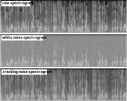
\includegraphics[width=\textwidth, keepaspectratio]{img/noise_spectrograms.png}
    	\caption{Spectrograms generated from the raw data, augmented with white noise and mixed with a cracking noise emulating analog telephony or a bad voice chat connection. The white noise aggressively subdues most higher frequencies and pauses causing a loss of classification performance. The cracking noise is less intrusive and therefore does not affect accuracy as much.}
    	\label{fig:noise}
	\end{figure}


Overall we note that even deep convolutional recurrent network are still subject to the influence of noise on audio. We learned that our spectrogram preprocessing does not help in these situations and that different network architectures play an instrumental role in dealing with these situations.
 
	\begin{table}[]
	\centering
	\begin{tabularx}{\textwidth}{lrrrrr}
	\toprule
	Dataset & \multicolumn{2}{c}{CRNN} & \multicolumn{2}{c}{Inception-v3 CRNN} \\  
                & Accuracy  & F1    & Accuracy  & F1   \\ \midrule
white noise     & 0.63      & 0.63  & 0.91      & 0.91 \\
cracking noise  & 0.82      & 0.83  & 0.93      & 0.93 \\
 	\bottomrule
	\end{tabularx}
	\caption{Accuracy and F1 score for our models evaluated on the speech data augmented with two different types of noise.}
	\label{tab:noise}
	\end{table}



\subsubsection{Background Music Robustness} 
\label{sec:music_robustness}
Many real world audio applications involve a some form of music. Therefore we evaluated our model to see if language identification was still possible when mixing speech with music. For this experiment we used two different test sets. For the first series we augmented our existing YouTube news dataset with randomly sampled background music in a similar fashion to the background noise augmentation. The background audio was obtained from Soundcloud\footnote{\url{https://soundcloud.com/royalty-free-audio-loops}, accessed 01.03.2017} and features royalty free, instrument-only music from various genres, including Pop, Dubstep, Rock and Electro amongst others. 
We volume normalized these sounds and overlaid them onto our speech data while trying to stay below the speech audio volume. In the best cases the two audio streams blend nicely with the background music producing a soft but noticeable ambient effect, while retaining the clarity of the speech. In other cases the audio levels and volume are over-accentuate for one or the other. The final result, however, does not resemble a complete song. We changed neither the tempo nor the pitch of our speaker and the rhythm of the vocals does not match the rhythm of the background audio. Therefore we gathered a small second test set of XXX \todo{insert number of songs} songs for each of the following genres: Pop, Rock, Hiphop, and Folk. 
Given that our training set does not intentionally include samples with music or songs we expected the performance do be drastically lower then for pure speech samples.

	\begin{table}[]
	\centering
	\begin{tabularx}{\textwidth}{lrrrr}
	\toprule
Dataset & \multicolumn{2}{c}{CRNN} & \multicolumn{2}{c}{Inception-v3 CRNN} \\   
                  & Accuracy  & F1    & Accuracy   & F1   \\ \midrule
Background Music  & 0.70      & 0.70  & 0.89  & 0.89 \\
Pop Songs         & 0.XX      & 0.XX  & 0.XX  & 0.XX \\
Rock Songs        & 0.XX      & 0.XX  & 0.XX  & 0.XX \\
HipHop Songs      & 0.XX      & 0.XX  & 0.XX  & 0.XX \\
Folk Songs        & 0.XX      & 0.XX  & 0.XX  & 0.XX \\

 	\bottomrule
	\end{tabularx}
	\caption{Accuracy and F1 score for our models evaluated on the speech data augmented background noise and songs sampled from four different genres.}
	\label{tab:audio_duration}
	\end{table}

\subsubsection{Model Extensibility} 
\label{sec:extensibility}
So far all our experiments were conducted on datasets consisting of only four languages: English, German, French and Spanish. We complemented these with two new languages spoken by millions around the globe: Mandarin Chinese and Russian. The goal of this experiment was to learn whether we could easily expand our model to other languages. 
We increased our existing YouTube news dataset with samples taken from Chinese and Russian news channels yielding the extended YouTube news dataset described in section \ref{sec:youtube_news}. In order to maintain the class distribution for six languages we had to decrease the number of training samples of the existing samples slightly. Table \ref{tab:dataset_comparison} contains the details for the extended YouTube news dataset.

For this approach we first finetuned our previous best CNN by replacing the final fully connected layers and adjusting the number of output nodes to accommodate for six classes. The resulting model served as the basis for training the CRNN in a similar manner as in earlier experiments. Applied on the test set we measured an accuracy of 0.92 and F1-score of 0.92. Both measurements match our previous evaluation with four languages on the YouTube news dataset as laid out in section \ref{sec:results_news} proving that the proposed CRNN architecture can easily be extended to cover more languages. Figure \ref{fig:6lang} shows individual performance measure of each language. Mandarin Chinese outperforms all other languages with a top accuracy of 0.96, which could be interpreted as it sounding the most contrasting to western languages and featuring its own unique intonation. We also noted that Russian was most frequently misclassified as Spanish and vice-versa. In contrast to our previous observation German is no longer the worst performing class, but English takes that role now. This is in part due to a significant number of misclassification as Russian samples.

	\begin{table}[]
	\centering
	\begin{tabularx}{\textwidth}{lrrrr}
	\toprule
     & accuracy & precision & recall  & F1 \\ \midrule
EN   & 0.86     & 0.89      & 0.88    & 0.88 \\
DE   & 0.89     & 0.91      & 0.90    & 0.90 \\
FR   & 0.93     & 0.94      & 0.93    & 0.94 \\
ES   & 0.92     & 0.91      & 0.93    & 0.92 \\
CN   & 0.96     & 0.97      & 0.96    & 0.96 \\
RUS  & 0.92     & 0.90      & 0.92    & 0.91 \\

 	\bottomrule
	\end{tabularx}
	\caption{}
	\label{tab:6lang}
	\end{table}

	\begin{figure}[]
  		\centering
    	\includegraphics[width=\textwidth, keepaspectratio]{plots/results_6lang_plot.pdf}
    	\caption{Individual performance measurements for each of our six target languages: English, German, French, Spanish, Mandarin Chinese, and Russian. Chinese exhibits the lowest misclassification rate while English performs the worst. Overall the model performance is consistent with previous evaluations on four languages as highlighted in section \ref{sec:results_news}.}
    	\label{fig:6lang}
	\end{figure}

Given that both new languages are rooted within their own respective language families and feature considerable different intonations we were content to find that the features learned by our model are indeed universal in nature. We are confident in the believe that the approach to language identification proposed in this these can be successfully applied to a wide variety of languages.

\subsubsection{Visualizations} 
\label{sec:visualization}
All previous sections described and evaluated our model by measuring various performance indicators and applying them to different datasets. In this section we will present plots underlining earlier observations from a different perspective.

First we visualized the high dimensional spectrogram embedding space using t-distributed stochastic neighbor embedding (\ac{tsne}) algorithm\cite{maaten2008visualizing}. t-SNE is a nonlinear dimensionality reduction technique employed to map high dimensional data into 2D or 3D space for plotting. We applied this machine learning algorithm to the first 2000 predictions of our second to last fully connected layer right before the classifier and managed to project our 1024 dimensional YouTube news data into a 2D space. Figure \ref{fig:tsne} shows the resulting plot highlighting a good separation of our four language classes as independent clusters confirming the network learned effective representations of the audio features. Note that French and Spanish split very nicely while German and English have some overlap. This is in line with our previous observations of classification errors as described in section \ref{sec:youtube_news}.

	\begin{figure}[h]
  		\centering
    	\includegraphics[width=\textwidth, keepaspectratio]{plots/tsne.pdf}
    	\caption{A 2D t-SNE plot of the high dimensional vector representation of our YouTube news samples. All four language classes from distinct clusters confirming the network learned effective representations of the audio features.}
    	\label{fig:tsne}
	\end{figure}

A primary advantage of deep neural networks is their ability to identify and learn useful feature by themselves making them powerful and versatile. From an end user's perspective they can appear as a bit of a black box and it remains unclear which features they ultimately deem relevant. In order to get a better understanding of our model we visualized its convolutional layers. In figure \ref{fig:conv_layer} we visualized some of the highest activating filters of the final convolutional layer. In order to obtain these filters we performed back propagation from the output of the filter we were interested in  back to an input image. This yielded the gradient of the output of the filter with respect to the input image pixels. We used that to perform gradient ascent, searching for the image pixels that maximize the output of the filter.

Visualizations for the lower level convolutional layers resulted in images of very simple geometric shapes like lines and circles which matched our expectations. With increasing network depth each convolutional layer's features combined and evolved into more complex shapes resembling our input domain. In our case we can identify the familiar ripple like patterns that form frequency activations over time. This proves that the network learned these structures as we hypothesized earlier. We can also identify that some filter specialize in high frequency whereas others focus on low frequencies. Furthermore, it can be observed that the filters only react to a short and specific span of time within the spectrogram, all of which are less than one second in duration.

	\begin{figure}[h]
  		\centering
    	
\includegraphics[width=\textwidth, keepaspectratio]{img/conv_filter.png}
    	\caption{Visualization of nine filters of the final convolutional layer. Note the ripple like patterns responsible for detecting different frequency spans in the input audio.}
    	\label{fig:conv_filter}
	\end{figure}

\subsubsection{Discussion and Comparison} 
\label{sec:comparison}

- evaluierung nur auf 10s snippets nd nicht auf ganzen audio files
- noch bessere perf mit majority voting über mehrere segmente
